\documentclass{beamer}
\usetheme{Warsaw}
\usecolortheme{seahorse}

\usepackage{graphicx}
\usepackage{subcaption}
\usepackage{csvsimple}
\usepackage{hyperref}

\newcommand*{\presentationgoldparispath}{../presentation_230120_gold2022_paris/fig/}%
\newcommand*{\mspath}{../../out/gwas417/pval_5e-08/r2_0.1/kb_1000/window_1000000/75_50}%
\newcounter{frame}[frame]
\setbeamertemplate{footline}[frame number]

% Change size of footnotes
\renewcommand{\footnotesize}{\fontsize{5pt}{5pt}\selectfont}
\title{Identification and analysis of pleiotropic expression quantitative trait loci}
\subtitle{CENTURI Scientific Day 2023}
\date{May 11, 2023 - Hexagone auditorium, Luminy campus}
\author{Aitor Gonz\'alez}
\institute{Aix Marseille Univ, INSERM, TAGC}

% Add section slide
\AtBeginSection[]
{
    \begin{frame}
        \frametitle{Table of Contents}
        \tableofcontents[currentsection]
    \end{frame}
}

\begin{document}

%%%%%%%%%%%%%%%%%%%%%%%%%%%%%%%%%%%%%%%%%%%%%%%%%%%%%%%%%%%%%%%%%%%%%%%%%%%%%%%%
    \begin{frame}

        \titlepage

    \end{frame}


    \section{Introduction} %%%%%%%%%%%%%%%%%%%%%%%%%%%%%%%%%%%%%%%%%%%%%%%%%%%%%%%%%%%%%%


%%%%%%%%%%%%%%%%%%%%%%%%%%%%%%%%%%%%%%%%%%%%%%%%%%%%%%%%%%%%%%%%%%%%%%%%%%%%%%%%
    \begin{frame}
        \frametitle{Genetic variants and diseases}

        \begin{itemize}
            \item Trait differences in human due to 80 x 10$^6$ genetic variants
            \item Genetic variants change susceptibilities to thousands of human traits
            \item For example, breast cancer:
        \end{itemize}
        %
        \begin{figure}
            \begin{center}
                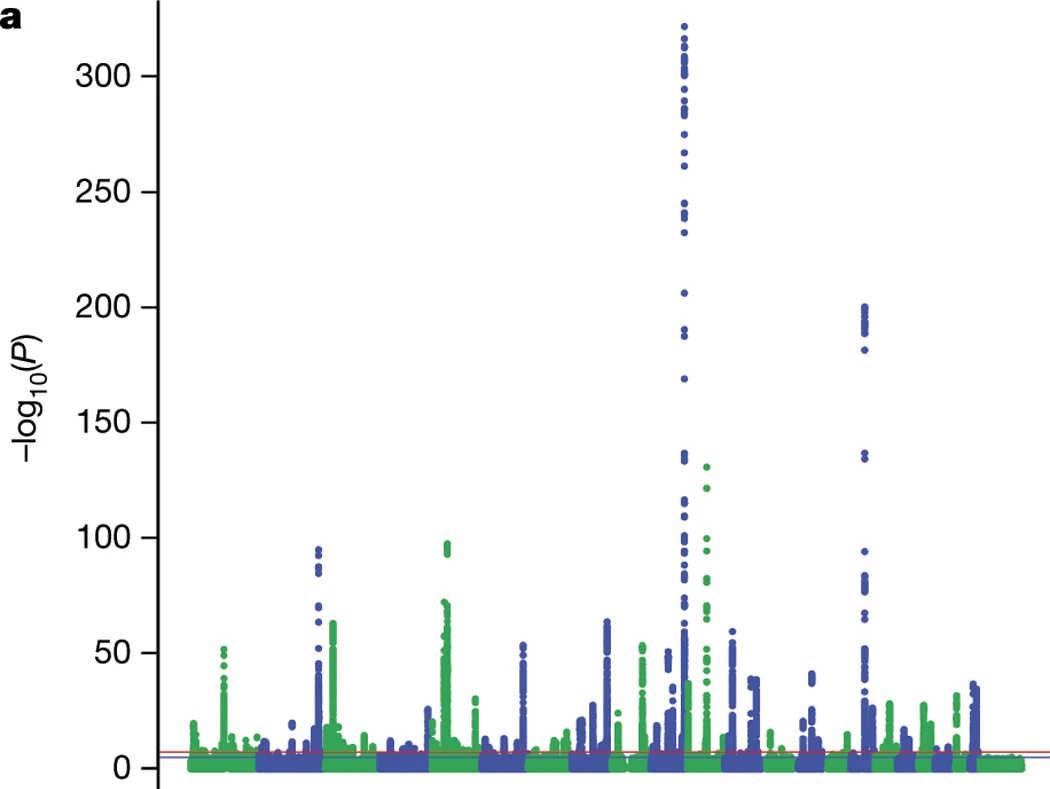
\includegraphics[width=0.5\textwidth]{\presentationgoldparispath/41586_2017_Article_BFnature24284_Fig1_HTML.jpg}
            \end{center}
            \caption{Genetic variant associations with breast cancer risk (DOI:10.1038/nature24284).}
        \end{figure}

        $\rightarrow$ What is the molecular mechanism of the trait association?

    \end{frame}

%%%%%%%%%%%%%%%%%%%%%%%%%%%%%%%%%%%%%%%%%%%%%%%%%%%%%%%%%%%%%%%%%%%%%%%%%%%%%%%%
    \begin{frame}
        \frametitle{eQTLs: Genetic variants that change gene expression}

        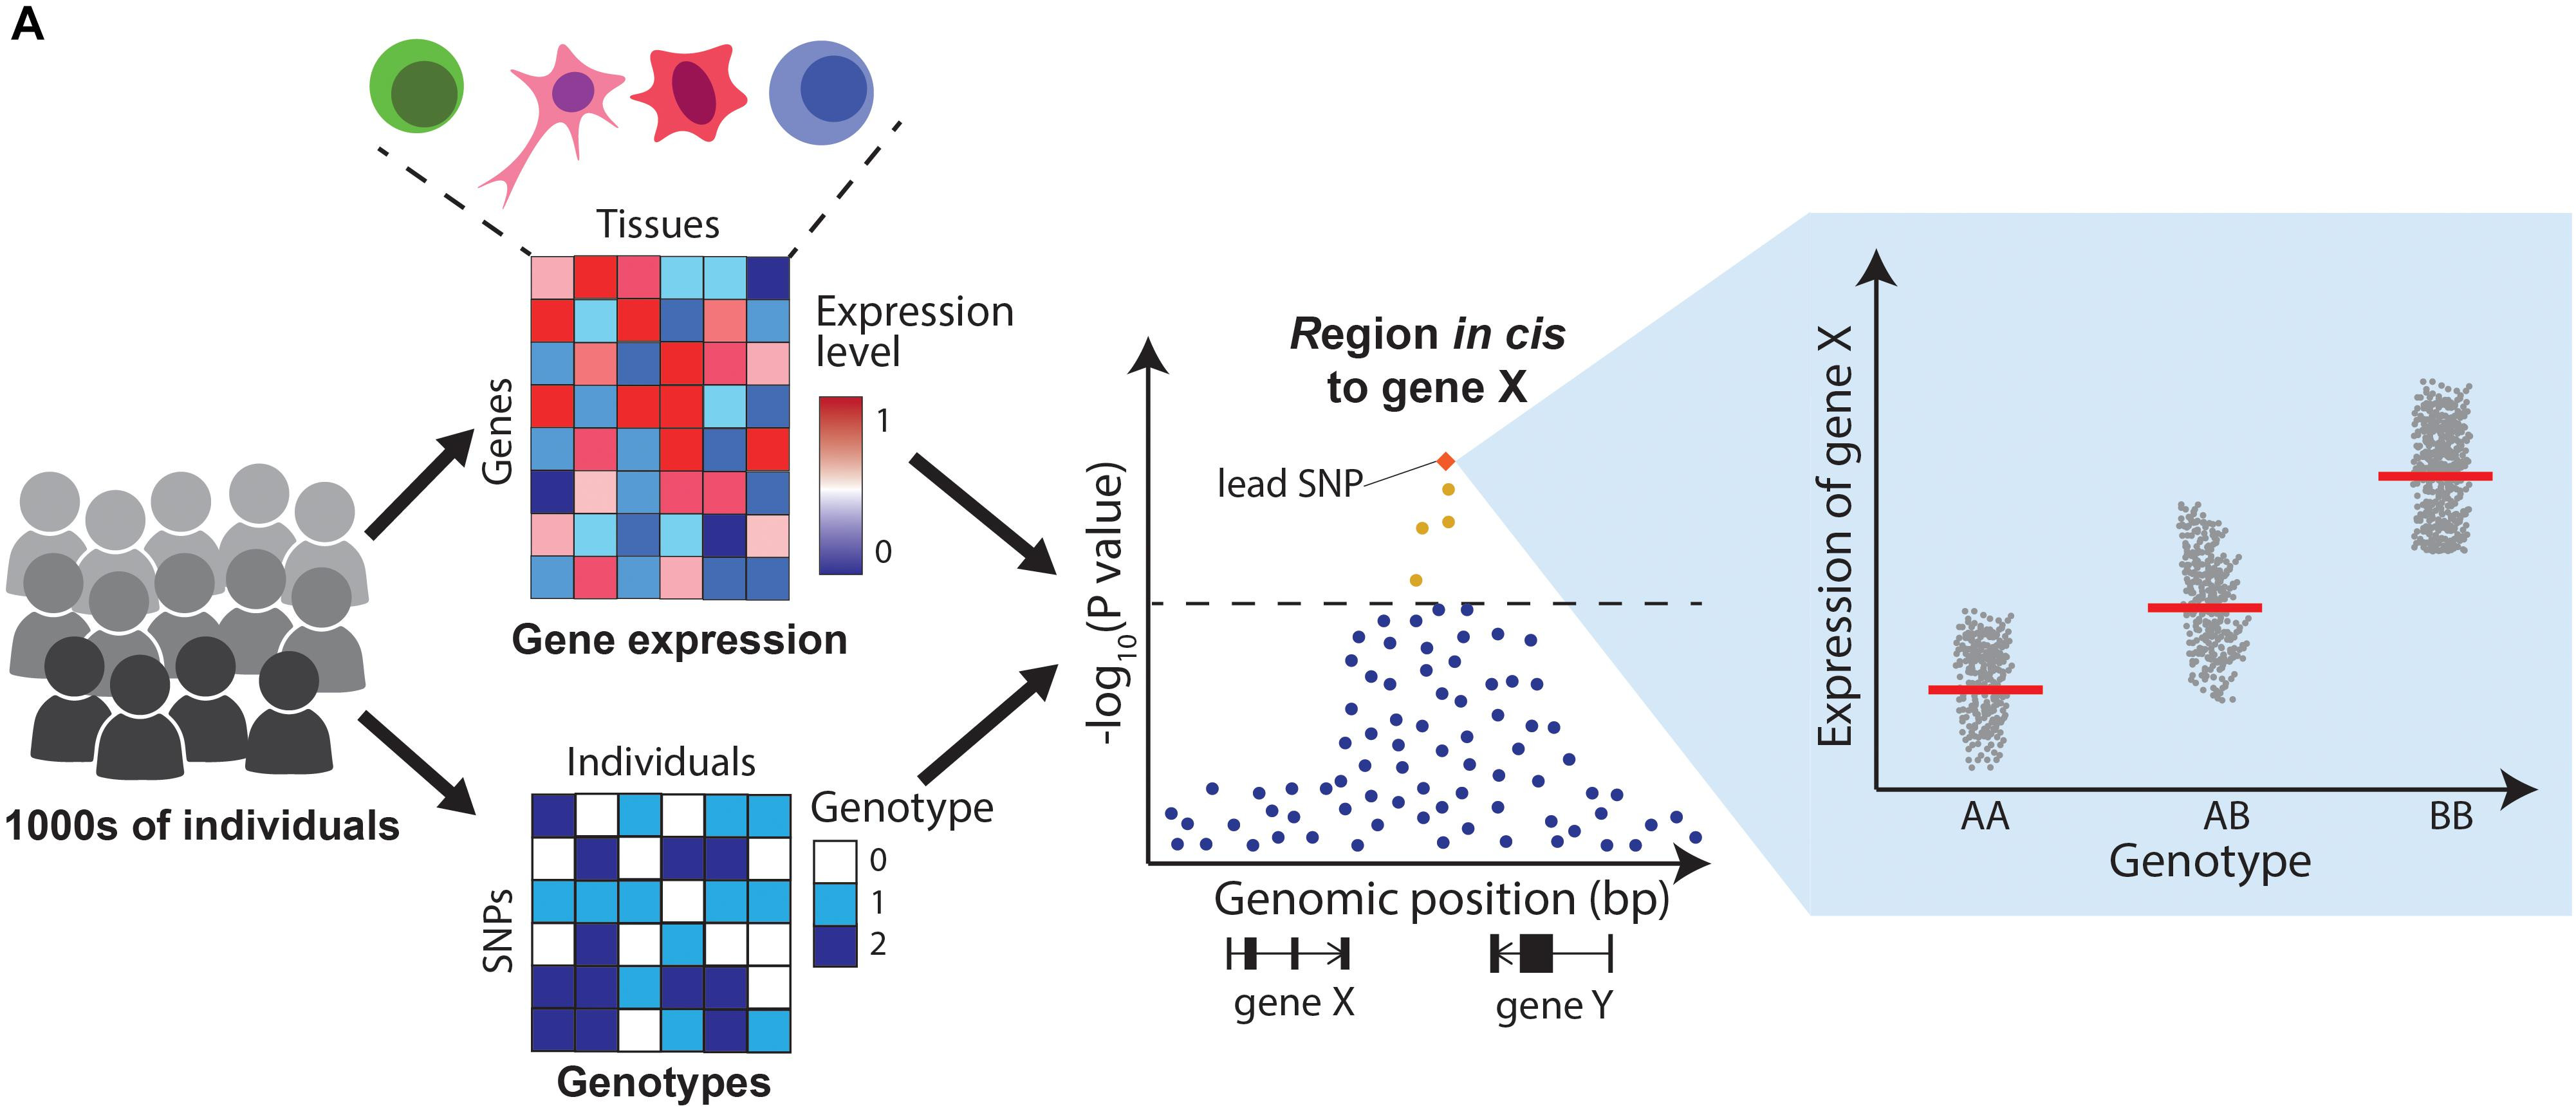
\includegraphics[width=0.7\textwidth]{\presentationgoldparispath/doi_10.3389_fgene.2020.00424_fig4a.jpg}

        \begin{itemize}
            \item eQTLs useful to indicate putative molecular mechanism of a trait variants
        \end{itemize}

        $\rightarrow$ How do we annotate trait variants with eQTLs?

        \let\thefootnote\relax\footnotetext{Cano-Gamez et al. 2020. doi:10.3389/fgene.2020.00424}
    \end{frame}

%%%%%%%%%%%%%%%%%%%%%%%%%%%%%%%%%%%%%%%%%%%%%%%%%%%%%%%%%%%%%%%%%%%%%%%%%%%%%%%%
    \begin{frame}
        \frametitle{Annotation of trait variants with eQTLs}

        $\rightarrow$ Colocalization of eQTLs and trait variants

        \begin{center}
            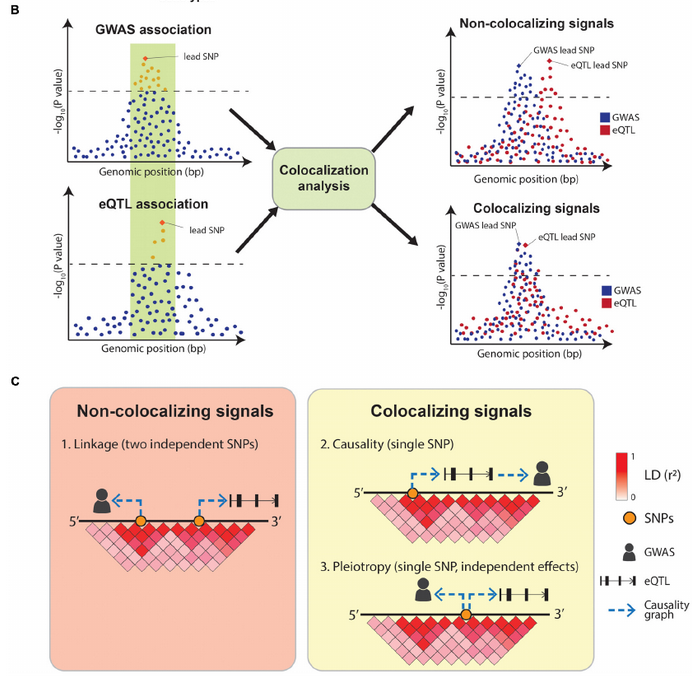
\includegraphics[width=0.5\textwidth]{\presentationgoldparispath/doi_10.3389_fgene.2020.00424_fig4bc.png}
        \end{center}

        \let\thefootnote\relax\footnotetext{Cano-Gamez et al. 2020. doi:10.3389/fgene.2020.00424}
    \end{frame}

%%%%%%%%%%%%%%%%%%%%%%%%%%%%%%%%%%%%%%%%%%%%%%%%%%%%%%%%%%%%%%%%%%%%%%%%%%%%%%%%
    \begin{frame}
        \frametitle{Pleiotropic genetic variants}

        \begin{itemize}
            \item Many genetic variants change simultaneously susceptibility to several diseases, for instance:
        \end{itemize}

        \begin{table}[!tbp]
            \centering
            \scriptsize
            \csvreader[separator=tab,
            tabular=crrcp{0.4\textwidth},
            late after last line=\\\hline,
            head,
            table head=\\\hline \bfseries Chrom. & \bfseries Pos (hg38) & \bfseries Ref. & \bfseries Alt. & \bfseries Trait categories\\\hline,
            ]{fig/count_per_rsid_gwas_ms.tsv}{}% use head of csv as column names
                {\csvcoli\ & \csvcolii\ & \csvcoliii\ & \csvcoliv\ & \csvcolvi}% specify your coloumns here
            \vspace{15pt}\label{tab:2}
        \end{table}

    \end{frame}

%%%%%%%%%%%%%%%%%%%%%%%%%%%%%%%%%%%%%%%%%%%%%%%%%%%%%%%%%%%%%%%%%%%%%%%%%%%%%%%%
    \begin{frame}
        \frametitle{Positioning of our work here in the state of the art}

        \begin{center}
            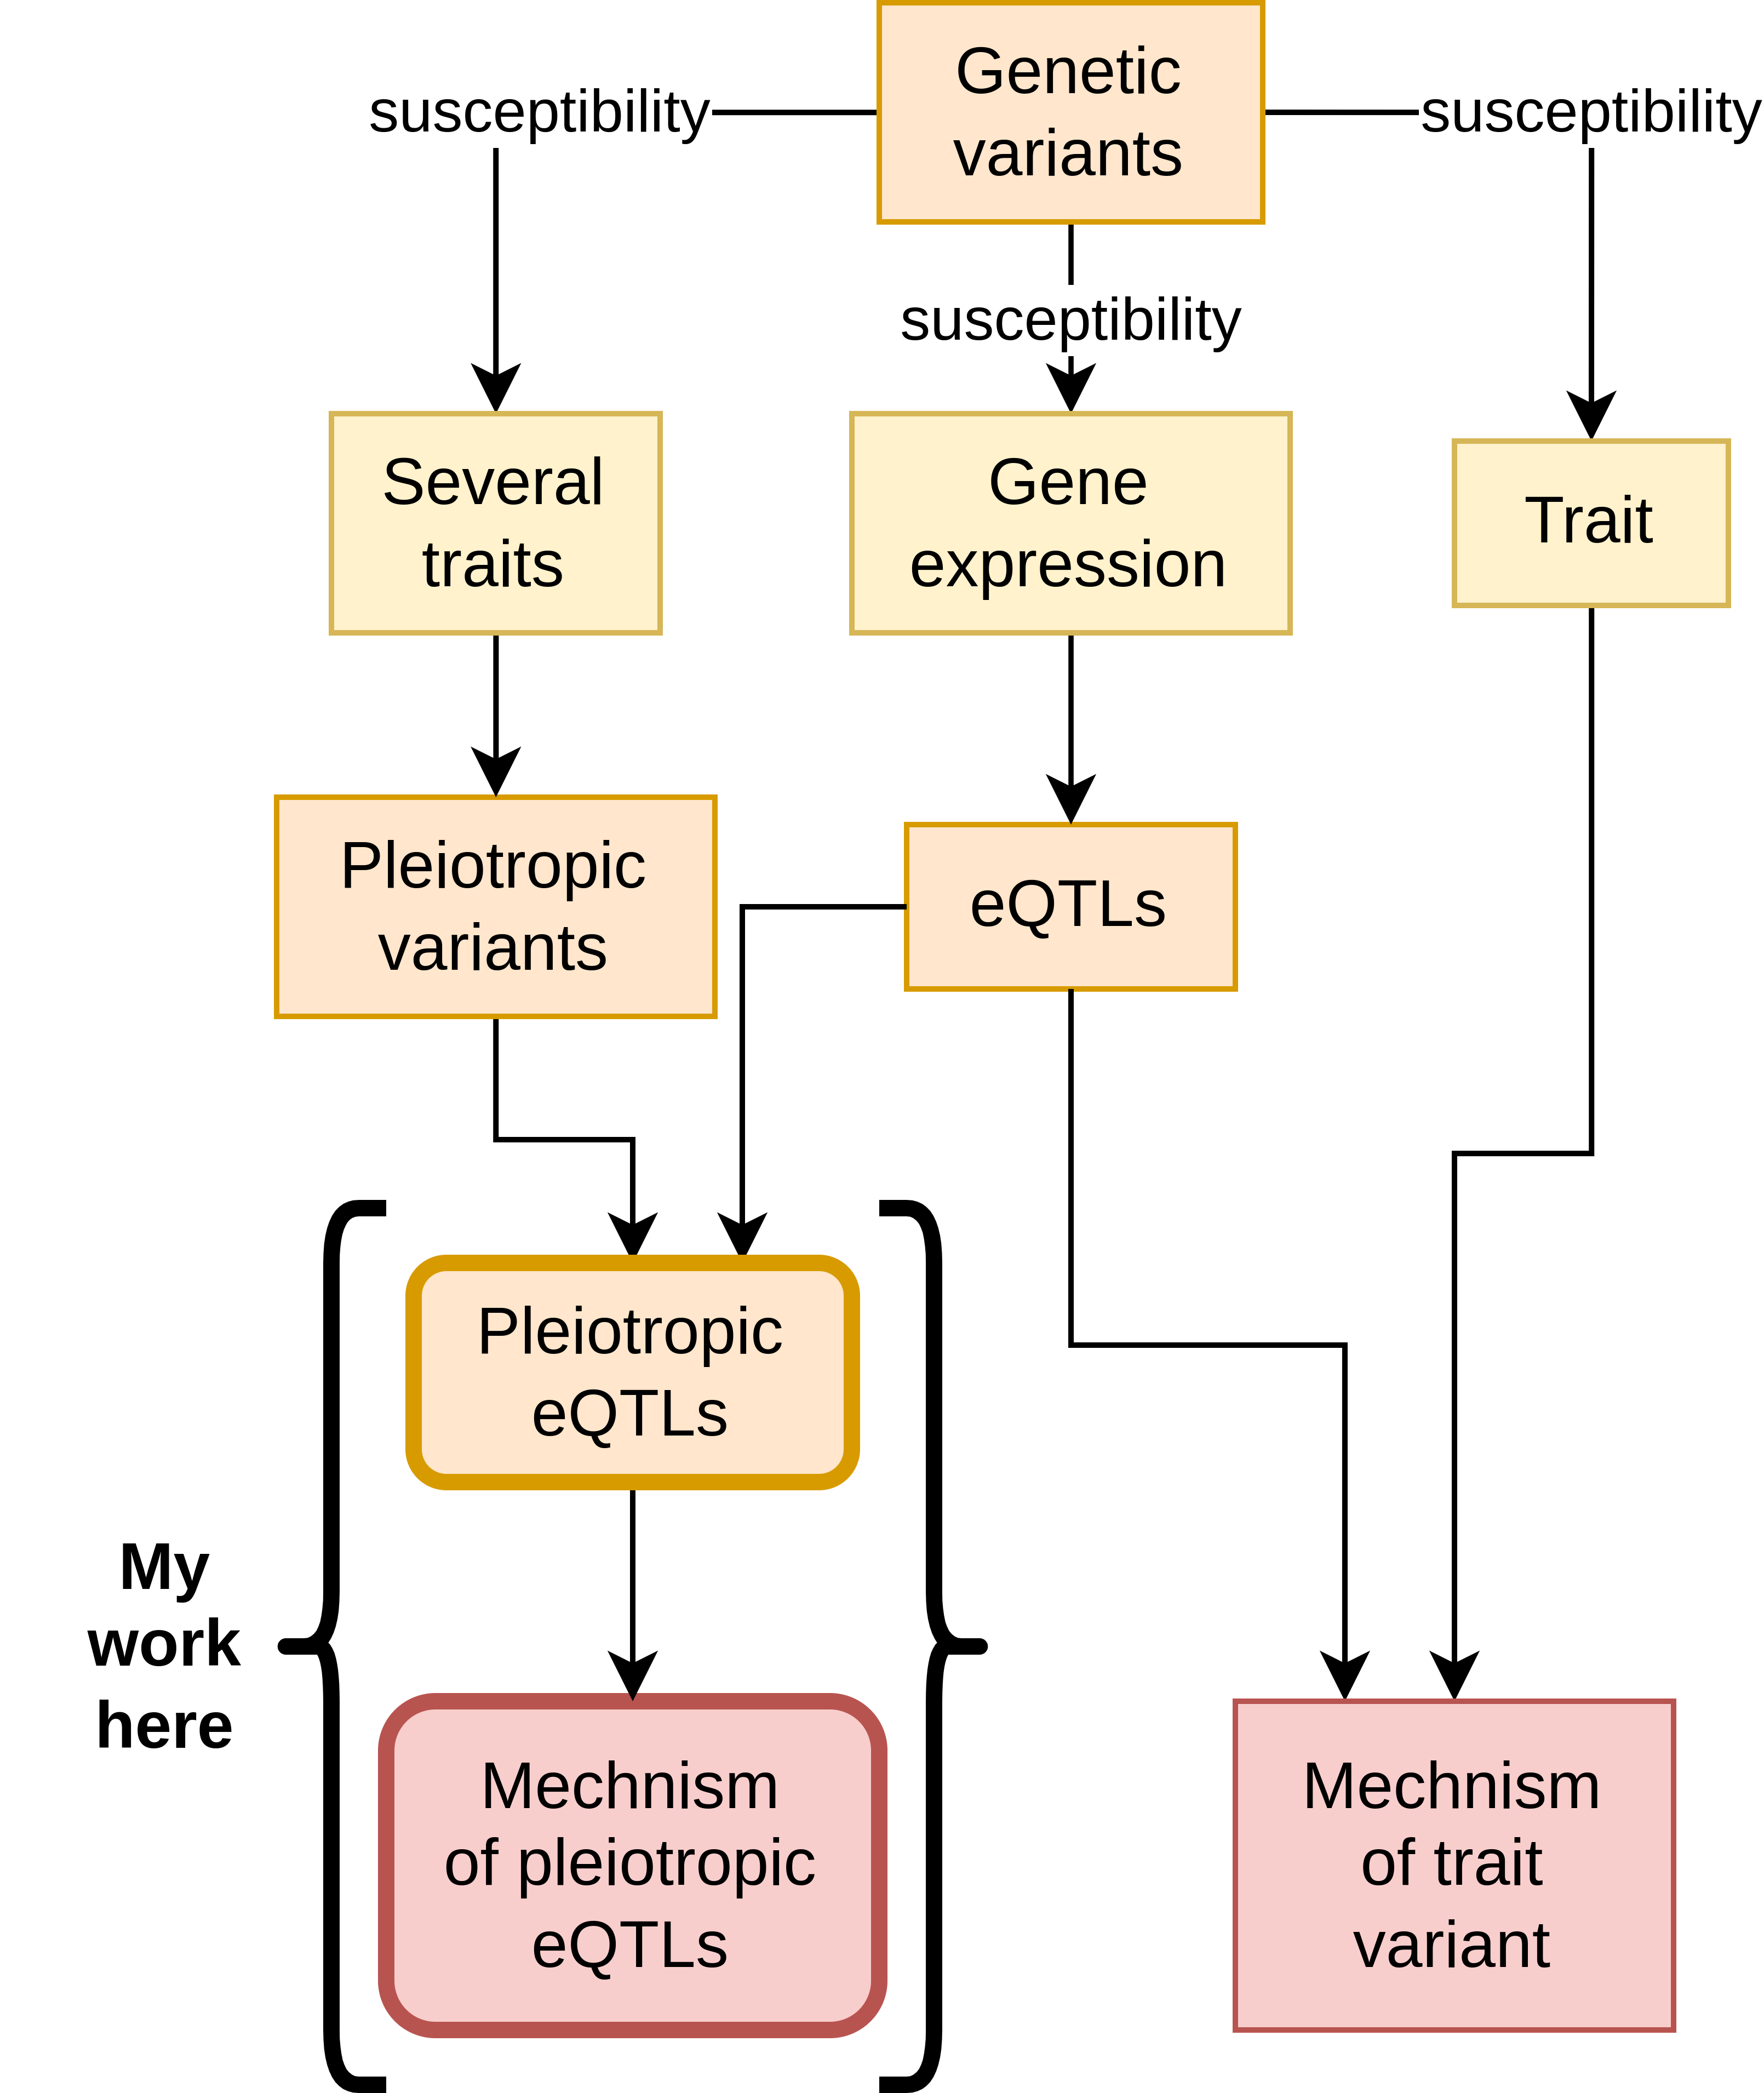
\includegraphics[width=0.6\textwidth]{fig/graphical_intro_approach.v2.drawio.png}
        \end{center}

    \end{frame}

%%%%%%%%%%%%%%%%%%%%%%%%%%%%%%%%%%%%%%%%%%%%%%%%%%%%%%%%%%%%%%%%%%%%%%%%%%%%%%%%
    \begin{frame}
        \frametitle{Strategy}

        \begin{enumerate}
            \item Compute colocalization of eQTLs and GWAS variants
            \item Split eQTLs by the number of associated disease categories
            \item Compare molecular properties of pleiotropic eQTLs
        \end{enumerate}

    \end{frame}


    \section{Results and discussion} %%%%%%%%%%%%%%%%%%%%%%%%%%%%%%%%%%%%%%%%%%%%%%%%%%%%%%%%%%%%%%

%%%%%%%%%%%%%%%%%%%%%%%%%%%%%%%%%%%%%%%%%%%%%%%%%%%%%%%%%%%%%%%%%%%%%%%%%%%%%%%%
    \begin{frame}
        \frametitle{Pleiotroic eQTLs}

        \begin{itemize}
            \item Analyzed: 138,274 variants from 293 traits and the 127 cell types/tissues
            \item Found: 476 pleiotropic eQTLs associated to $\geq$ two traits categories
            \item Important genomic regions: ABO, ALDH2, IL4, TP53, ...
        \end{itemize}

        \begin{table}[!tbp]
            \centering
            \scriptsize
            \csvreader[separator=tab,
            tabular=crrrcp{0.4\textwidth},
            late after last line=\\\hline,
            head,
            table head=\\\hline \bfseries Chrom. & \bfseries Pos (hg38) & \bfseries Ref. & \bfseries Alt. & \bfseries Gene marker& \bfseries Trait categories\\\hline,
            ]{fig/count_per_rsid_gwas_ms.tsv}{}% use head of csv as column names
                {\csvcoli\ & \csvcolii\ & \csvcoliii\ & \csvcoliv\ & \csvcolv\ & \csvcolvi}% specify your coloumns here
            \vspace{15pt}\label{tab:1}
        \end{table}

    \end{frame}

%%%%%%%%%%%%%%%%%%%%%%%%%%%%%%%%%%%%%%%%%%%%%%%%%%%%%%%%%%%%%%%%%%%%%%%%%%%%%%%%
    \begin{frame}
        \frametitle{Is the effect size of pleiotropic eQTLs different?}

        \begin{figure}[!ht]

            \begin{subfigure}[]{.49\textwidth}
                \textbf{a}
                \\
                \includegraphics[width=\textwidth]{\mspath/pltbar_x_per_gwas_cat_y_beta_neglog10pval.py/eqtl_beta.png}
            \end{subfigure}
            %
            \begin{subfigure}[]{.49\textwidth}
                \textbf{b}
                \\
                \includegraphics[width=\textwidth]{\mspath/pltbar_x_per_gwas_cat_y_beta_neglog10pval.py/gwas_beta.png}
            \end{subfigure}

        \end{figure}
        %
        \vfill
        Yes, pleiotropic eQTLs have a lower effect on gene expression and traits

    \end{frame}

%%%%%%%%%%%%%%%%%%%%%%%%%%%%%%%%%%%%%%%%%%%%%%%%%%%%%%%%%%%%%%%%%%%%%%%%%%%%%%%%
    \begin{frame}
        \frametitle{Are pleiotropic eQTLs closer to genes?}

        \begin{center}
            \includegraphics[width=0.5\textwidth]{\mspath/plt_x_per_variant_y_egene_distance.py/violin.png}
        \end{center}
        \vfill
        Yes, distance to genes decreases with the pleiotropy

    \end{frame}

%%%%%%%%%%%%%%%%%%%%%%%%%%%%%%%%%%%%%%%%%%%%%%%%%%%%%%%%%%%%%%%%%%%%%%%%%%%%%%%%
    \begin{frame}
        \frametitle{Are pleiotropic eQTLs associated to more genes?}

        \begin{center}
            \includegraphics[width=0.5\textwidth]{\mspath/pltbar_x_per_variant_etissue_y_egene.py/plt.png}
        \end{center}
        \vfill
        Yes, number of target gene increases with the pleiotropy

    \end{frame}

%%%%%%%%%%%%%%%%%%%%%%%%%%%%%%%%%%%%%%%%%%%%%%%%%%%%%%%%%%%%%%%%%%%%%%%%%%%%%%%%
    \begin{frame}
        \frametitle{A web portal to access the eQTL/trait annotations}

        \url{https://gwas2eqtl.tagc.univ-amu.fr/gwas2eqtl}

        \begin{center}
            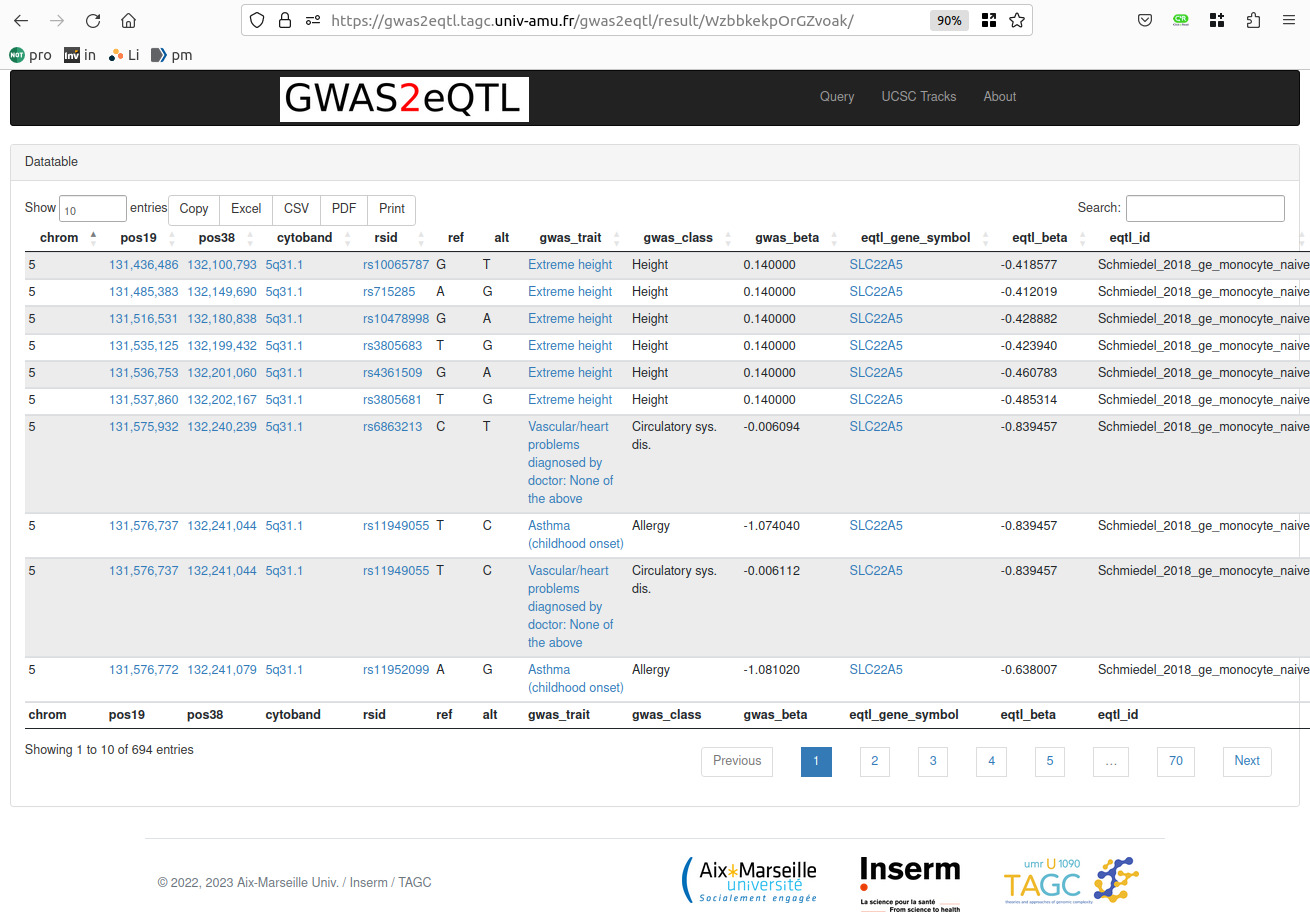
\includegraphics[width=0.9\textwidth]{fig/gwas2eqtl.png}
        \end{center}

    \end{frame}

%%%%%%%%%%%%%%%%%%%%%%%%%%%%%%%%%%%%%%%%%%%%%%%%%%%%%%%%%%%%%%%%%%%%%%%%%%%%%%%%
    \begin{frame}
        \frametitle{Graphical summary}

        \begin{center}
            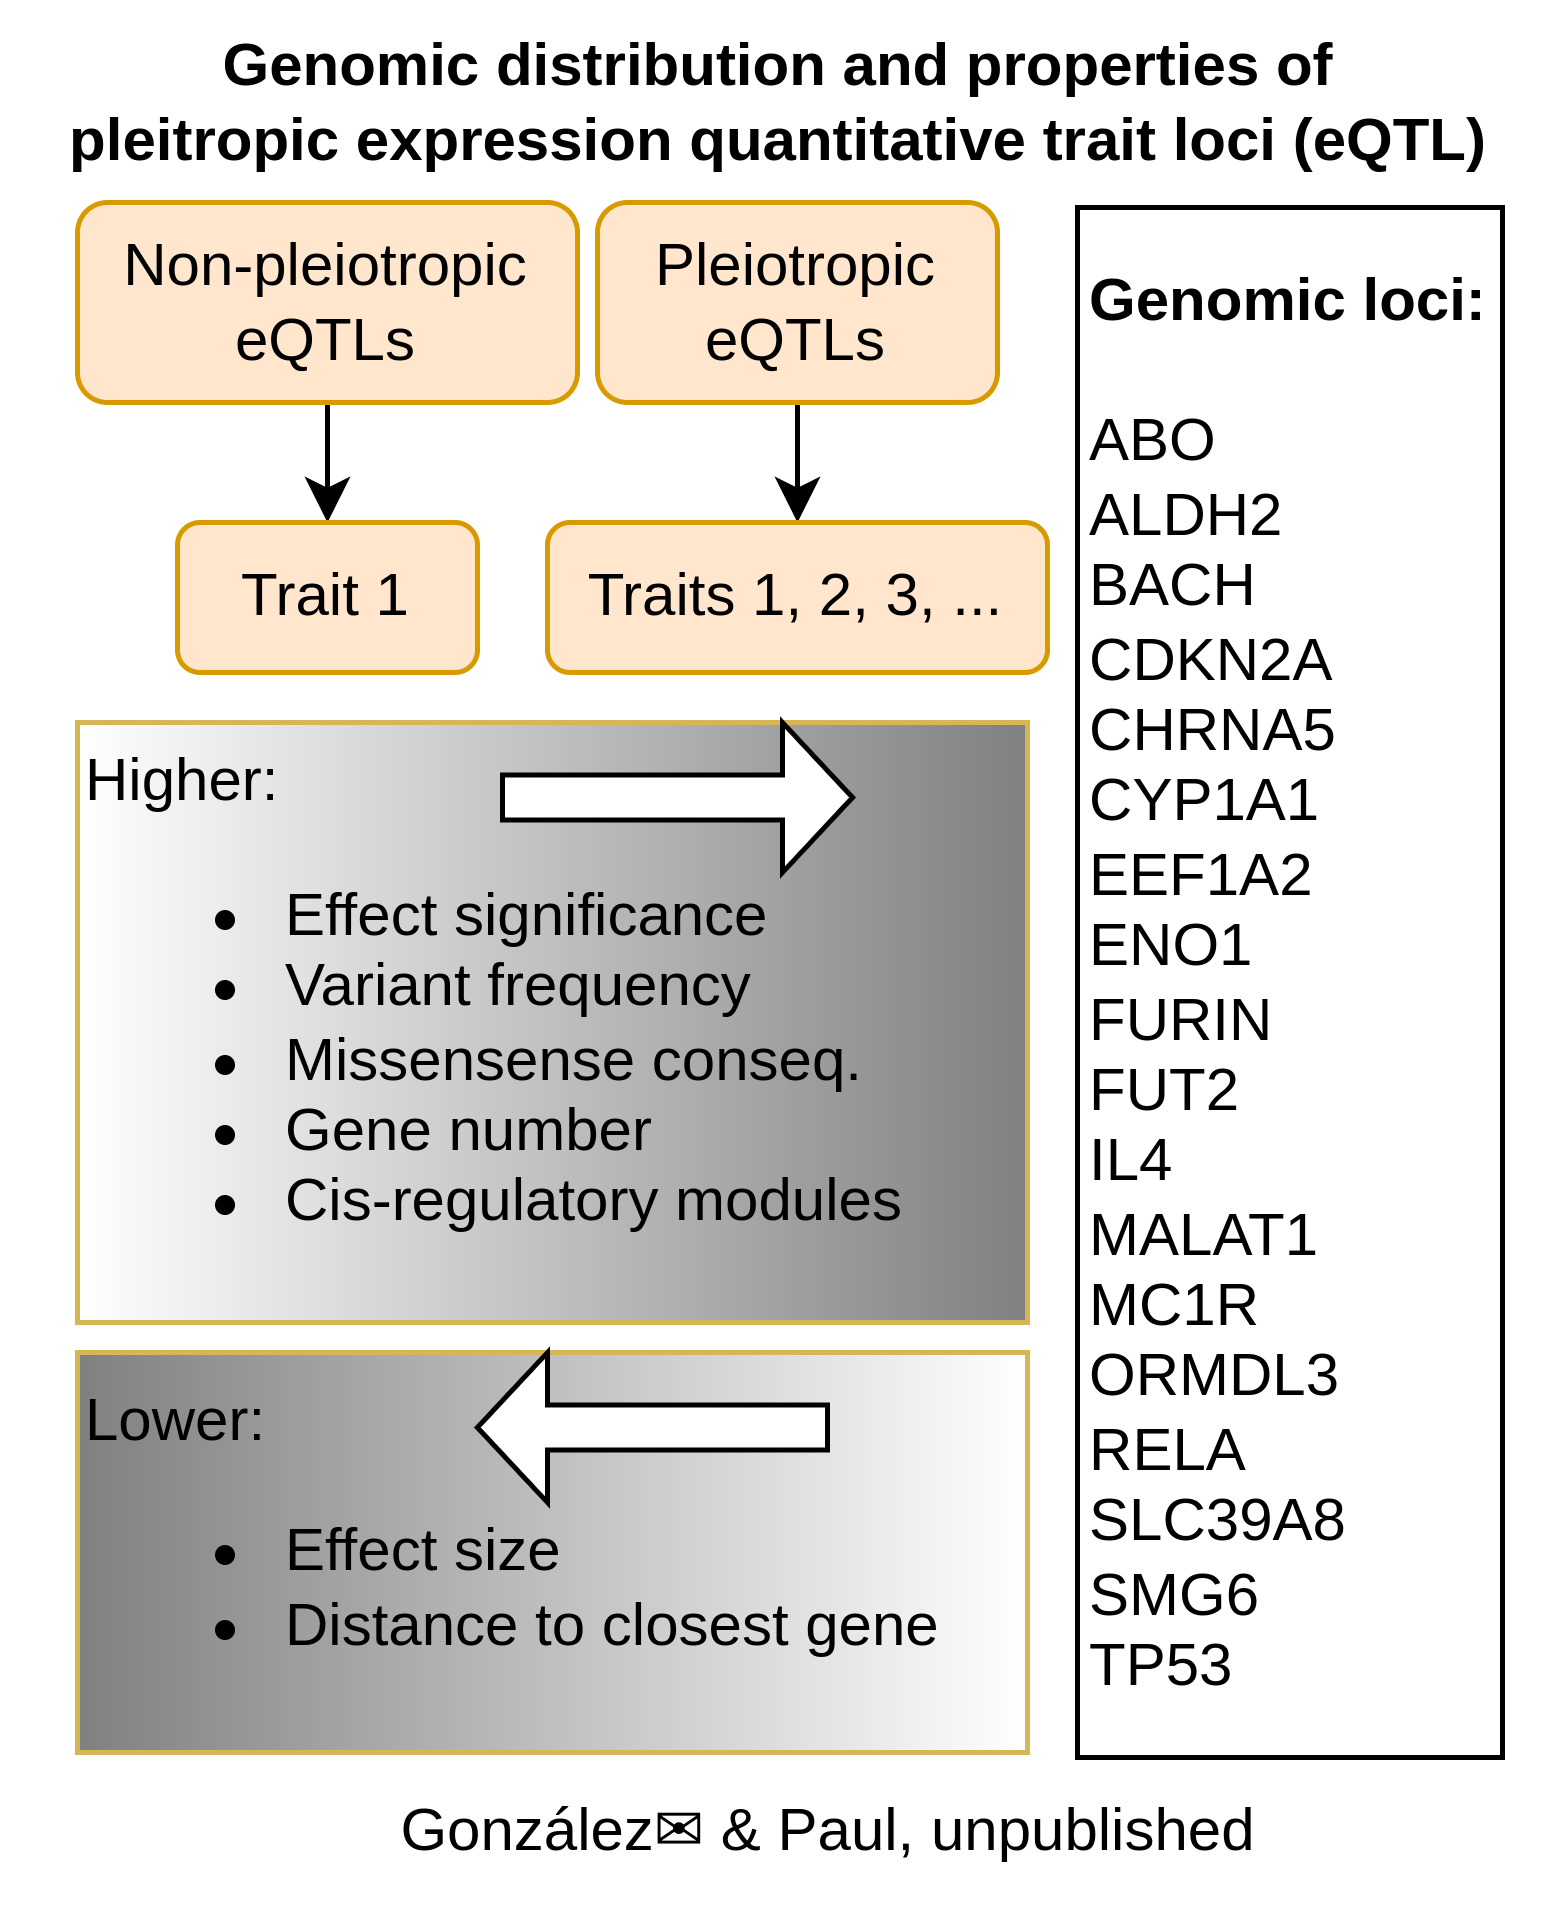
\includegraphics[width=0.6\textwidth]{fig/graphical_abstract.drawio.png}
        \end{center}

    \end{frame}

%%%%%%%%%%%%%%%%%%%%%%%%%%%%%%%%%%%%%%%%%%%%%%%%%%%%%%%%%%%%%%%%%%%%%%%%%%%%%%%%
    \begin{frame}
        \frametitle{
\includegraphics[width=0.1\textwidth]{fig/opentonetwork.png} Applications of these datasets}

        \begin{itemize}
            \item Large dataset of genetic variants ...
            \item ... associated to traits and gene expression changes in 127 tissues and cell types
            \item Useful to annotate genomic regions and genes
        \end{itemize}

    \end{frame}

%%%%%%%%%%%%%%%%%%%%%%%%%%%%%%%%%%%%%%%%%%%%%%%%%%%%%%%%%%%%%%%%%%%%%%%%%%%%%%%%
    \begin{frame}
        \frametitle{Acknowledgements}

%
        Collaborators and colleagues at TAGC, specially:
        %
        \begin{itemize}
            \item P. Paul, L. Lecerf (M1), P. Rihet, M. Michel, S. Marquet, S. Spicuglia.
        \end{itemize}
%
        \vfill
%
        Funding and resources:
%
        \begin{itemize}
            \item Institut Cancer et Immunologie - Aix-Marseille Univ.
            \item Agence nationale de la recherche (ANR)
            \item Centre de Calcul Intensif d'Aix-Marseille
        \end{itemize}
%
        \vfill
        %
        Thank you for your attention!!

    \end{frame}

\end{document}
